\part{Tutorial}

\chap{Your First Robotics Project}\label{ch.intro}

\sect{Getting to know your Thymio}

\Cref{fig.front} shows the front and top of Thymio. On the top you
can see the center circular button (\textcolor{blue}{A}) and four
directional buttons (\textcolor{blue}{B}). Behind the buttons, the green
light (\textcolor{blue}{C}) shows how much charge remains in the
battery. At the back are the top lights (\textcolor{blue}{D}), which
have been set to red in this picture. There are similar lights on the
bottom (see \cref{fig.bottom}). The small black rectangles
(\textcolor{blue}{E}) are sensors which you will learn about in
\cref{ch.pet}.

\begin{figure}[h]
\begin{center}
\gr{front}{.8}
\caption{The top and front of the Thymio robot}\label{fig.front}
\end{center}
\end{figure}

\sect{Connect the robot and run VPL}

Connect your Thymio robot to your computer with a USB cable; the robot
will play a sequence of tones. If the robot is turned off, turn it on by
touching the center button for a few seconds until you hear the tones.
Run VPL by double-clicking on the icon \blksm{thymiovpl} on your
computer.

\importantbox[Small images]{When a small image appears
in the text, a larger image is displayed in the margin.}

VPL may connect automatically to your robot. If not, the window shown in
\cref{fig.connect} will be displayed. Check the box next to \bu{Serial},
click on \bu{Thymio Robot} below it, select a language, and then click
\bu{Connect}. Depending on the configuration of your computer and
operating system, there may be several entries in this table and the
data following \bu{Thymio Robot} may be different from what is shown in
the Figure.

\trickbox{It is also possible to access VPL from Aseba Studio, the
text-based programming environment through the VPL plugin found in the
\textit{Tool} area at the bottom left of the screen.}

\begin{figure}
\begin{center}
\gr{connect}{.4}
\caption{Connect to Thymio through serial port (USB)}\label{fig.connect}
\end{center}
\end{figure}

\newpage

\sect{The VPL user interface}

The user interface of VPL is shown below.
There are six areas in the interface:
\begin{enumerate}[noitemsep,nosep]
\item A toolbar with buttons for opening, saving, running a program, etc.
\item A program area where programs for controlling the robot are constructed.
\item A message area which displays error messages if the program is not
well-formed.
\item A column with event blocks for constructing your program.
\item A column with action blocks for constructing your program.
\item The translation of the program into AESL, the textual language of Aseba.
\end{enumerate}

\plainfloat
\begin{figure}[h]
\gr{gui}{1}
\caption{The VPL window}\label{fig.vplgui}
\end{figure}
\framedfloat

\bigskip

\informationbox{To go further}{ When you construct a program using VPL, the
translation of the program into the textual programming language AESL
appears in the right part of the window. It is the AESL program that is
actually run by the robot. If you are curious and wish to understand
AESL, you can read the \cref{ch.next} which explains these translations.
Then, go to
\href{https://www.thymio.org/en:asebausermanual}{https://www.thymio.org/en:asebausermanual}
for learning and reference materials on AESL and its Studio
environment.}

\newpage

\sect{Write a program}

When you start VPL, a blank program area is displayed.

If, after having built a piece of program, you wish to clear the content
of the program area, click \blksm{new} (\bu{New}).

A program in VPL consists of \emph{event-actions pairs}, each
constructed from an event block and one or more action blocks. For
example, the pair: \blkc{e-a-pair} causes the top light of the robot to
display red when the front button is touched.

\importantbox[Meaning of an event-actions pair]{\centering When the event
occurs, the associated actions are run.}

The program area will initially contain an empty frame for an
event-actions pair: \blkc{empty-frame} To bring a block to the program
area from the columns (areas 4 and 5 of \cref{fig.vplgui}), press and
hold the left mouse button and drag the block to a dashed square. When the
block is over the square, release the mouse button, dropping the block
into its place.

\importantbox{The technique just described is call
\emph{drag-and-drop} and is widely used in the user interface of
programs.}

Start by bringing the button event block \blksm{event-buttons} into the
left side of the empty frame. You will get a message inviting you to add
an action block. Drag the top color action block
\blksm{action-colors-up} and drop it into the right side of the frame. You have
constructed an event-actions pair!

Next, we have to modify the event and the action to do what we want. For
the event, click on the front button (the top triangle); it will turn
red: \blkc{forward} This specifies that an event will occur when the
\textit{front button} of Thymio is touched.

The color action block contains three \emph{sliders}---colored bars with
a white square---one for each of the primary colors red, green, blue.
Drag a white square to the right and then back to the left, and you will
see that the background color of the block changes. All colors can be
made by mixing these three primary colors: red, green and blue. Move
the red slider until the square is at the far right, and move the green
and blue sliders until they are at the far left. The color will be all
red with no blue nor green: \blkc{red}

\sect{Save the program}

Before running the program, save it on your computer. Click on the
button \blksm{save} (\bu{Save}) in the toolbar. You will be asked to
give the program a name; choose a name that will help you remember what
the program does, perhaps, \bu{display-red}. Choose the location where
you want to save your program and click on \bu{Save}.


\importantbox[Save frequently]{When you modify a program, click
\bu{Save} frequently so that you don't lose your work if something
happens to the computer.}


\sect{Run the program}

To run the program, click on \blksm{run} (\bu{Run}) in the toolbar.
Touch the front button on the robot; the light on top of the robot
should change to red.

\informationbox{Congratulations!}{You have created and run your
first program. Its behavior is:\\ \textbf{When you touch the forward
button of the Thymio, it becomes red.}}

If you need to stop the VPL program, click \blksm{stop} (\bu{Stop}) .
This is important when you run a program that causes the robot to move,
but the program does not have an event-actions pair to stop the motors.

\sect{Turn the robot off}

When you have finished working with the Thymio robot, you can turn it
off by touching and holding the center button for a few seconds until
you hear a sequence of tones. The battery in the robot will
continue charging as long as it is connected to a working computer. A
red light next to the USB cable connector means that the robot is
charging; it turns blue when the charging is completed (\cref{fig.back}).
You can disconnect the cable when you are not using the robot.

\trickbox{You can charge the robot faster by using a mobile phone
charger with a micro-USB connector.}

\begin{figure}
\begin{center}
\gr{back}{.6}
\caption{The back of the Thymio showing the USB cable and the
 charging light}\label{fig.back}
\end{center}
\end{figure}

Should the USB cable disconnect during programming, VPL will wait for
the connection to be made again. Check both ends of the cable, reconnect
and see if VPL is working. If you have a problem, you can always close
VPL, reconnect the robot and open VPL again.

%\newpage

\sect{Modify a program}

\begin{itemize}

\item To delete an event-actions pair, click \blkxsm{x} at the top-right
of the pair.

\item To add an event-actions pair, click \blkxsm{plus} available below
an existing pair.

\item To move an event-actions pair to another position in the program,
drag and drop it at the desired location.

\item To copy an event-actions pair to another position in the program,
press and hold the \bu{Ctrl} and then use the mouse to drag and drop the
pair at the desired location.\label{p.copy-pairs}\footnote{On Mac
OS, the \bu{Command} button is used instead of \bu{ctrl}.}

\end{itemize}

\informationbox{The blinking \bu{Run} button}{When you modify a program,
the \bu{Run} button blinks blue and green to remind you that you need to
click the button to load the modified program into the Thymio
robot.\label{p.blink}}

If you want to experiment with a modification but not lose an existing
program, you can create a copy of the existing program by clicking
\blksm{saveas} (\bu{Save as}) and giving a new file name.

\sect{Open an existing program}

Suppose that you have saved your program and turned off the robot and
the computer, but later you wish to continue to work on the program.
Connect the robot and run VPL as described previously. Click on
\blksm{open} (\bu{Open}) and select the program you want to open, for
example, \bu{display-red}. The event-actions pairs of the program will
be displayed in the program area, and you can continue working on it.

\newpage

\sect{The current event-actions pair}

When you click on an event-actions pair, it will be displayed with a
yellow background. This will also occur when you enter an event or
action block in an empty pair:

\begin{center}
\begin{tabular}{c@{\hspace{.1\textwidth}}c}
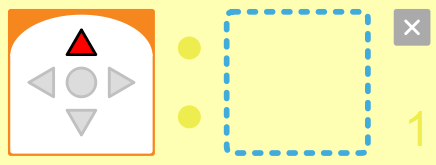
\includegraphics[width=.3\textwidth,keepaspectratio=true]{event-action-pair-yellow1}
&
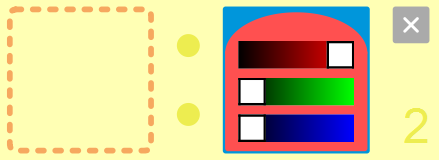
\includegraphics[width=.3\textwidth,keepaspectratio=true]{event-action-pair-yellow2}
\end{tabular}
\end{center}

The left gold-colored square is the space for the event; the right
blue-colored square is for the first (or only) action. The pair with the
yellow background is called the \emph{current} pair.

\informationbox{Quick entering of a block}{If you click on an event or action block, it will be
automatically placed in the program area in the current
event-actions pair.}

\bigskip

\bigskip

\informationbox{The VPL toolbar}{\cref{a.toolbar} contains a
description of all the buttons in the VPL toolbar. Look at it
occasionally until you have learned how to use them.}
